A partir da descrição das características do SAD SustenAgro (seção
\ref{sec:SAD-SustenAgro}), do requisito de modelar o conhecimento
através de ontologias (usando tecnologias da Web Semântica) e de definir
uma DSL para facilitar a definição de comportamentos por parte dos
especialistas, foi modelado e desenvolvido um protótipo de um framework,
intitulado Decisioner, que permite definir e gerar SADs do tipo do
SustenAgro. O framework Decisioner é basicamente formado por ontologias,
que representam conhecimento do domínio, e por uma DSL que permite
definir comportamentos e estabelecer configurações gerais de um SAD.

Satisfazer os requisitos requeridos pelos pesquisadores da Embrapa
Meio Ambiente foi uma das forças que dirigiram o desenvolvimento desta
pesquisa. Para chegar a arquitetura, aqui apresentada, houve um trabalho
interativo para chegar aos requisitos que eram gerais, que deveriam
estar no framework, e os que eram específicos, que deveriam estar
definidos na ontologia ou na DSL do SustenAgro. 

Neste capítulo será apresentado a arquitetura do protótipo Decisioner,
cada uns dos seus componentes e funcionalidades e as contribuições
para esta pesquisa.

\section{Arquitetura do Decisioner}

Os SADs, segundo a descrição feita no capítulo \ref{chap:SAD}, são
compostos por banco de dados, base de conhecimento, módulo de processamento
da informação e módulo gerador de resultados. Em cada um desses módulos,
está implícito o conhecimento dos especialistas, pelo qual a primeira
característica definida do Decisioner foi a integração de ontologias. 

As ontologias permitem a definição do conhecimento dos especialistas
em um componente independente. Ele é complementado pela DSL, que permite
definir comportamento e características do SAD. O diagrama para a
arquitetura desenvolvida para essa solução é apresentado na figura
\ref{fig:Componente-DSL}. Com base nesse diagrama, os componentes
dos SADs foram generalizados e, por meio do desenvolvimento de experimentos,
foi definida uma arquitetura que pode ser reusada em diferentes SADs
(do mesmo tipo do SustenAgro).

O Decisioner pode ser classificado como um framework. Já que é uma
plataforma de software com design reutilizável e implementações reutilizáveis
pelos clientes, que o especializam em um domínio particular \citep{RiehlePhdthesis}.

A arquitetura do framework Decisioner é composta pelos componentes
gerais para a definição de SADs, apresentados na Figura \ref{fig:Interfaces}.
Usuários especialistas podem interagir com o framework através dos
editores de ontologias e DSL. Usuários finais interagem através da
sua interface Web.

\begin{figure}[H]
\centering{}\includegraphics[width=0.9\columnwidth]{\string"figures/Decisioner Architecture\string".eps}\caption{Arquitetura do Decisioner\label{fig:Interfaces}}
\end{figure}

Os componentes dessa arquitetura são:
\selectlanguage{english}%
\begin{enumerate}
\item \textbf{Domain ontology}\foreignlanguage{brazil}{: representa os conceitos
específicos dos especialistas que serão utilizados no SAD.}
\item \textbf{Decisioner ontology}\foreignlanguage{brazil}{: faz uma ligação
entre os tipos de dados e as interfaces gráficas capazes de mostrar
ou editar esses dados, fazendo um mapeamento entre os dois.}
\item \textbf{Ontology Editor}\foreignlanguage{brazil}{: componente que
permite editar as ontologias em um formato mais fácil para o uso pelos
especialistas.}
\item \textbf{Triplestore}\foreignlanguage{brazil}{: sistema de armazenamento
e recuperação da informação em formato de triplas }RDF\foreignlanguage{brazil}{,
(explicado em detalhe na seção \ref{subsec:Triplestore}). Ele permite
o gerenciamento de dados e ontologias em formato }RDF.\foreignlanguage{brazil}{
A traves da linguagem padrão }SPARQL Protocol and RDF Query Language
(Sparql)\foreignlanguage{brazil}{ \citep{prud2006sparql}. }
\item \textbf{DSL code}\foreignlanguage{brazil}{: representa uma instancia
da DSL com as definições particulares para um SAD específico.}
\selectlanguage{brazil}%
\item \textbf{DSL Editor}: Editor visual web da DSL com recursos como \foreignlanguage{english}{code
completion} e \foreignlanguage{english}{syntax coloring}. Permite
a edição da \foreignlanguage{english}{DSL} por parte dos especialistas
do domínio.
\selectlanguage{english}%
\item \textbf{Web components}:\foreignlanguage{brazil}{ conjunto de elementos
visuais que podem ser reusados nos SADs com a finalidade de modularizar
e simplificar a geração de }Web User Interfaces\foreignlanguage{brazil}{
(UI\nomenclature{UI}{User Interface}).}
\item \textbf{DSL Interpreter}\foreignlanguage{brazil}{: Interpretador
da DSL para processar as definições do SAD e criar um SAD específico.
Ele usa a DSL, ontologias e componentes web para gerar automaticamente
a interface e comportamento de um SAD específico.}
\item \textbf{Web UI}\foreignlanguage{brazil}{: Interfaces visuais geradas
pelo }DSL Interpreter.\foreignlanguage{brazil}{ Utilizam os }Web Components\foreignlanguage{brazil}{
e fornecer a interface gráfica, usadas pelos usuários finais, na interação
com o SAD na Web.}
\end{enumerate}
\selectlanguage{brazil}%
Essa arquitetura foi implementada em um protótipo Decisioner. Sempre
que possível, na implementação do Decisioner, foram reutilizados componentes
ou bibliotecas disponíveis publicamente na internet.

\section{Metodologia}

Com a finalidade de desenvolver o protótipo do framework Decisioner,
escolheu-se o SAD SustenAgro como um caso de uso e exemplo de instanciação.
Ele permitiu a definição de uma metodologia de desenvolvimento para
os componentes. Teria sido interessante instanciar o framework para
um segundo SAD, para demonstrar melhor sua generalidade. Contudo,
dada as limitações de tempo impostas a um trabalho de mestrado e ao
tempo necessário ao desenvolvimento do framework, isso não foi possível.
No decorrer deste texto, foram feitas algumas considerações sobre
a generalidade do framework. A metodologia abordada durante este processo,
incluiu as seguintes etapas:
\begin{enumerate}
\item Seleção da \foreignlanguage{english}{Triplestore}: foram avaliadas
as \foreignlanguage{english}{triplestores} existentes com a finalidade
de definir uma que se adaptasse aos requisitos do framework.
\item Seleção da linguagem de programação e framework web: foi realizada
uma verificação das tecnologias de desenvolvimento de sistemas web
compatíveis com as tecnologias da web semântica e com a \foreignlanguage{english}{DSL}.
\item Design da DSL: Durante o processo de desenvolvimento do SAD SustenAgro,
foram generalizados seus componentes, permitindo definir cada uma
das características da DSL. O processo foi iterativo, permitindo refinar
a expressividade da linguagem com a ajuda de especialistas da Embrapa.
\item Desenvolvimento do \foreignlanguage{english}{DSL editor}: implementação
de uma \foreignlanguage{english}{web UI} que permite editar a DSL
em formato textual, fornecendo aos especialistas um editor moderno.
Modificações na DSL podem ser vistas no SAD imediatamente.
\item Desenvolvimento do \foreignlanguage{english}{Ontology Editor}: implementação
de uma \foreignlanguage{english}{web UI} com componentes específicos
para suportar a edição das ontologias, por parte dos especialistas,
em um formato textual.
\item Desenvolvimento do \foreignlanguage{english}{DSL Interpreter}: o interprete
da Decisioner DSL. Esse componente tinha que ser atualizado a medida
que o design da DSL mudava.
\item Integração com \foreignlanguage{english}{web components} e \foreignlanguage{english}{web
UI}s: \foreignlanguage{english}{Widgets} gráficas, na forma de \foreignlanguage{english}{Web
components} suportam a geração das \foreignlanguage{english}{Web UIs}
que compõem os SADs. \foreignlanguage{english}{Widgets} foram adicionadas
para atender as necessidades do SustenAgro.
\end{enumerate}
A metodologia de desenvolvimento foi guiada pelo desenvolvimento do
SAD SustenAgro. Primeiramente foram desenvolvidas as ontologias, continuando
com o desenvolvimento do \foreignlanguage{english}{DSL Interpreter}
e depois com a integração dos \foreignlanguage{english}{web components}
e \foreignlanguage{english}{UI}s. Foram realizados vários ciclos de
desenvolvimento para refinar as funcionalidades. A Figura \ref{fig:Metodologia-do-Decisioner}
representa a metodologia realizada.

\begin{figure}
\begin{centering}
\includegraphics[width=0.9\columnwidth]{\string"figures/Decisioner Methodology\string".eps}
\par\end{centering}
\caption{Metodologia de desenvolvimento do Decisioner\label{fig:Metodologia-do-Decisioner}}

\end{figure}

A seguir, cada componente da arquitetura do Decisioner é discutido,
começando pela ontologia Decisioner.

\section{Ontologia Decisioner\label{sec:Ontologia-Decisioner}}

Para desenvolver um protótipo de uma ontologia geral, que abstraísse
os conceitos dos SADs, foram analisados os sistemas SAD desenvolvidos
pela Embrapa Meio Ambiente, descritos na seção \ref{sec:SAD-SustenAgro}.

A versão inicial da ontologia foi modelada na ferramenta Protégé,
no formato \foreignlanguage{english}{OWL}. Depois foi criado um novo
formato, usando o \foreignlanguage{english}{YAML Ain't Markup Language
(YAML \nomenclature{YAML}{YAML Ain't Markup Language\\})}, mais simples
que \foreignlanguage{english}{OWL}, para ser usado pelos especialistas
no \foreignlanguage{english}{Ontology Editor}, explicado na seção
\ref{sec:Ontology-Editor}.

A ontologia Decisioner contém os elementos comuns identificados e
abstraídos dos SADs da Embrapa, e tem o proposito de fornecer uma
ontologia geral que dê suporte a SADs diferentes. 

\begin{figure}[H]
\centering{}\includegraphics[scale=0.7]{\string"figures/DSS ontology\string".eps}\caption{Modelagem abstrata do SAD\label{fig:Modelagem-do-SAD}}
\end{figure}

Na Figura \ref{fig:Modelagem-do-SAD}, é apresentada a hierarquia
de classes resultante. Ela contém as classes:
\selectlanguage{english}%
\begin{description}
\item [{Evaluation\ Object\foreignlanguage{brazil}{:}}] \foreignlanguage{brazil}{classe
que representa os objetos que serão analisados em cada processo de
avaliação. Eles serão indivíduos dessa classe ou de alguma subclasse
dela.}
\item [{Feature\foreignlanguage{brazil}{:}}] \foreignlanguage{brazil}{classe
que representa as caraterísticas a avaliar em um }Evaluation Object.\foreignlanguage{brazil}{
Elas serão quantificadas, analisadas e usadas no processo de geração
de relatórios no processo de avaliação. As }Features\foreignlanguage{brazil}{
têm associado um }Value\foreignlanguage{brazil}{ que as quantifica.
Existe a subclasse }\textit{Weighted}\foreignlanguage{brazil}{ que
representa uma }Feature\foreignlanguage{brazil}{ vinculada a um peso.
Esse peso pode ser usado nas fórmulas para o cálculo dos modelos codificados
pelos especialistas.}
\item [{Place\foreignlanguage{brazil}{:}}] \foreignlanguage{brazil}{classe
que representa a localização física dos objetos modelados, permitindo
referenciar geograficamente um }Evaluation Object.
\item [{Analysis\foreignlanguage{brazil}{:}}] \foreignlanguage{brazil}{classe
que representa uma avaliação associada a um }Evaluation Object\foreignlanguage{brazil}{.
Suas instâncias têm propriedades, como nome e data da avaliação, e
correspondem a uma avaliação cadastrada.}
\item [{Value\foreignlanguage{brazil}{:}}] \foreignlanguage{brazil}{classe
que representa os valores que são atribuídos a cada instância de }Feature.\foreignlanguage{brazil}{
As subclasses }Real\foreignlanguage{brazil}{ e }Categorical\foreignlanguage{brazil}{
representam tipos de valores.}
\item [{User\foreignlanguage{brazil}{:}}] \foreignlanguage{brazil}{classe
que representa os usuários do sistema.}
\item [{Role\foreignlanguage{brazil}{:}}] \foreignlanguage{brazil}{classe
que representa os papéis de usuário do sistema e suas permissões.
Por padrão, estão instanciados os perfis }User\foreignlanguage{brazil}{
e }Admin.
\end{description}
\selectlanguage{brazil}%
A partir dessas classes é possível organizar os conceitos específicos
de cada SAD como subclasses delas. Um aspecto importante das ontologias
é que suportam a inferência de novos conhecimentos, permitindo classificar
e relacionar dados novos do sistema, ajudando desta maneira na automatização
da geração dos SADs. Isso permite ao \foreignlanguage{english}{DSL
Interpreter} mapear qualquer conceito novo, específico de um SAD em
particular, a um desses conceitos conhecidos e saber o que deve ser
feito com ele. 
\selectlanguage{english}%

\section{Ontology Editor\label{sec:Ontology-Editor}}

\selectlanguage{brazil}%
Para suportar a edição das ontologias do domínio, por parte dos especialistas,
foi implementado um editor web. Ele permite editar a ontologia específica
do SAD em um formato baseado em \foreignlanguage{english}{YAML,} a
descrição da ontologia neste formato passa a um conversor para ficar
no formato \foreignlanguage{english}{OWL} que é processado pela \foreignlanguage{english}{API}
de protégé para instanciar a ontologia com as restrições definidas
e finalmente exportado como \foreignlanguage{english}{RDF} para ser
substituído na \foreignlanguage{english}{triplestore} \foreignlanguage{english}{Blazegraph,}
este processo é realizado a cada vez que o usuário salva a ontologia.

A Figura \ref{fig:Editor-de-ontologia} mostra uma imagem do editor.
Ela mostra o código da ontologia em formato \foreignlanguage{english}{YAML},
um \foreignlanguage{english}{side panel,} que apresenta as classes,
propriedades e indivíduos hierarquicamente (permitindo a referenciação
dos elementos no código), um \foreignlanguage{english}{button restore}
para restituir a ultima versão da ontologia e um \foreignlanguage{english}{button
save} para salvar e carregar no Decisioner a ontologia em edição.

Idealmente, especialistas de domínio deveriam poder criar a ontologia
usando um editor gráfico. Mas devido as restrições de escopo de um
projeto de mestrado, não haveria tempo para criar um. A criação de
uma ferramenta, como um editor gráfico, teria o escopo de um novo
mestrado. 

Usar um editor para \foreignlanguage{english}{OWL}, como o Protégé,
exigiria que os especialistas de domínio aprendessem \foreignlanguage{english}{OWL}
e lógica descritiva, o que não é uma opção viável. Este editor de
ontologias é uma solução intermediária. Ele adota um formato em \foreignlanguage{english}{YAML},
menos complexo que \foreignlanguage{english}{OWL}, mas expressivo
o suficiente para as necessidades das ontologias. Ele ajuda os usuários
a encontrar os elementos da ontologia (\foreignlanguage{english}{side
panel}) e permite a inserção da ontologia no Decisioner. Apesar de
ser possível aos especialistas desenvolver uma ontologia totalmente
nova, usando o editor, seu objetivo é permitir que eles possam fazer
modificações localizadas nas ontologias. 
\begin{flushleft}
\begin{figure}[H]
\begin{centering}
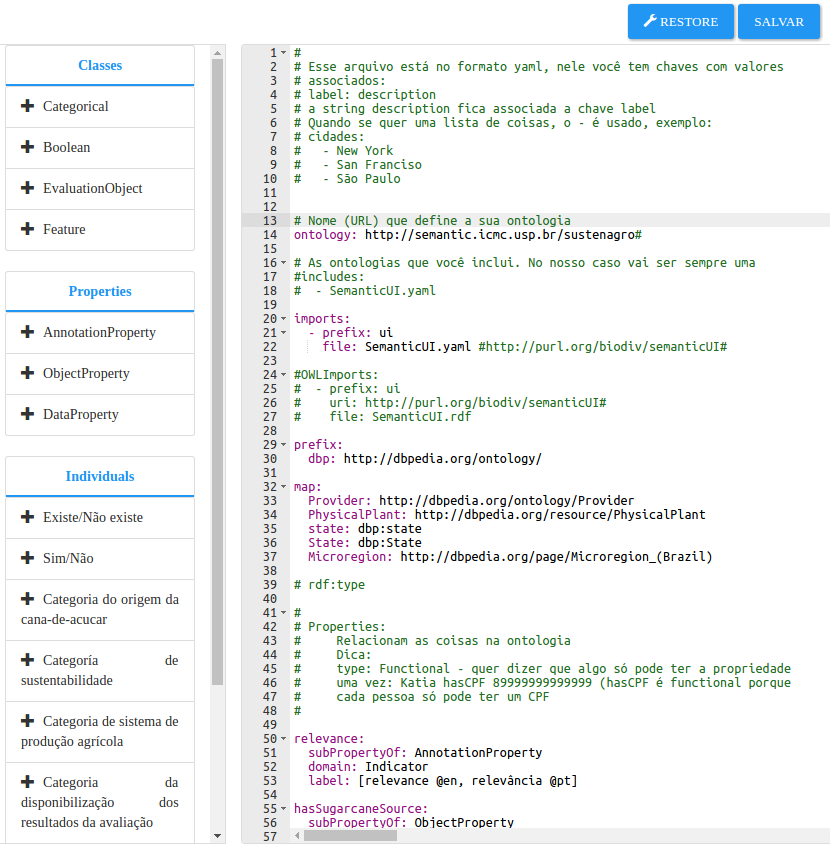
\includegraphics[width=1\columnwidth]{figures/SustenAgro-ontology-editor}
\par\end{centering}
\caption{Editor de ontologia\label{fig:Editor-de-ontologia} }
\end{figure}
\par\end{flushleft}

A ontologia definida em este editor será usada para definir a estrutura
dos SADs, as funcionalidades dos SADs são descritas na DSL apresentada
a continuação. 

\section{Decisioner DSL}

Para permitir que os especialistas definam o comportamento do framework
Decisioner, foi definida uma DSL que permite definir as principais
características de um SAD. Tal DSL foi baseada na modelagem geral
da arquitetura do \foreignlanguage{english}{Decisioner} e permite
relacionar conceitos específicos dos especialistas, criar equações
para os modelos usados, gerar a interface web para o usuário final,
servindo de interface entre a ontologia do Decisioner e a ontologia
do domínio.

A DSL foi baseada na linguagem \foreignlanguage{english}{Groovy},
porque ela suporta o desenvolvimento de \foreignlanguage{english}{DSLs}
que se comportam como extensões da linguagem \foreignlanguage{english}{Groovy}.

O uso da DSL, por parte especialistas, diminui o esforço necessário
no desenvolvimento de um SAD. Ela permite que os próprios especialistas
sejam capazes de fazer parte do desenvolvimento e validação do SAD.
Especialmente na parte de refinamento e atualização do SAD, especialistas
podem fazer modificações no sistema sem a ajuda de programadores e
ver o resultado dessas mudanças imediatamente.

As instruções definidas na DSL são:
\selectlanguage{english}%

\subsection*{Evaluation Object}

\selectlanguage{brazil}%
Nos SAD focados na avaliação, existe um objeto de avaliação que representa
as entidades a serem avaliadas. Esse objeto é constituído por propriedades
que especificam o que está sendo avaliado. A instrução \foreignlanguage{english}{\textit{evaluationObject}}\textit{
}permite definir as propriedades desse objeto. Por exemplo, caso uma
fazenda esteja sendo avaliada, é possível criar propriedades como
nome, tipo de produção, localização, etc.

A instrução tem como argumentos a URI (ou label) da classe da ontologia
do domínio, que será objeto de avaliação, e cada uma das propriedades
relacionadas. O algoritmo \ref{alg:Defini=0000E7=0000E3o-do-Evaluation}
apresenta um exemplo que usa a classe \textit{ProductionUnit}, como
classe dos objetos a serem avaliados e define as propriedades \textit{hasName},
para nome, e \textit{hasAgriculturalProductionSystem}, para tipo de
produção. Podem ser usados os labels das propriedades, ao invés de
suas URIs\textit{.}

\begin{algorithm}[H]
\inputencoding{latin9}\begin{lstlisting}
evaluationObject ":ProductionUnit", {     
 instance "ui:hasName', label: ["en": "Name", "pt": "Nome"]
 instance ":hasAgriculturalProductionSystem"
 type label: ["en": "Type", "pt": "Tipo"]
}
\end{lstlisting}
\inputencoding{utf8}
\caption{Definição do Evaluation Object\label{alg:Defini=0000E7=0000E3o-do-Evaluation}}
\end{algorithm}

O comando \foreignlanguage{english}{\textit{instance}} vincula uma
propriedade definida na ontologia, através da URI. Ela pode ser complementada
por parâmetros que customizam a representação visual da propriedade.
O comando \foreignlanguage{english}{\textit{type}} faz com que os
\foreignlanguage{english}{EvaluationObject} tenham que ser de subclasses
da classe principal. Por exemplo, uma unidade produtiva pode ser uma
plantação greenfield (mecanizada e uniforme), fazenda familiar, etc.
Os parâmetros que podem complementar as instruções anteriores são:
\selectlanguage{english}%
\begin{enumerate}
\item \textit{required}\foreignlanguage{brazil}{: define uma propriedade
obrigatória}
\item \textit{label}\foreignlanguage{brazil}{: define um texto associado}
\item \textit{placeholder}\foreignlanguage{brazil}{\textit{:} define um
texto de ajuda}
\item \textit{widget}\foreignlanguage{brazil}{: define um controle gráfico
de usuário}
\end{enumerate}

\subsection*{Feature}

\selectlanguage{brazil}%
A instrução \foreignlanguage{english}{\textit{Feature}} define as
características, do Evaluation Object, que serão usadas na sua avaliação.
O DSL Interpreter vai gerar uma interface gráfica, onde o usuário
final terá que preencher os dados sobre cada característica. Cada
característica tem um tipo associado a ela (na ontologia de domínio).
A partir dele, é possível associar uma widget específica para edição.
Por exemplo, a Figura \ref{fig:Widgets-geradas-da-DSL} mostra a
widget para uma característica que tem um tipo categórico com 3 possíveis
valores. Os textos mostrados vêm da ontologia e fazem parte da descrição
de cada elemento. É possível criar descrições em mais de uma língua.

\begin{figure}[H]
\begin{centering}

\includegraphics[width=0.8\columnwidth]{figures/IndicatorSelection}
\par\end{centering}
\caption{Widget geradas a partir da definição da DSL\label{fig:Widgets-geradas-da-DSL}}
\end{figure}

Quando o usuário final usa a widget, o valor escolhido é anotado,
no Evaluation Object, usando a propriedade \foreignlanguage{english}{\textit{has
value}}. Nas fórmulas, usadas para os cálculos do modelo usado, é
possível acessar esses valores. Os usuários não precisam preencher
a todas as características.

\begin{algorithm}[H]
\inputencoding{latin9}\begin{lstlisting}
feature ':EnvironmentalIndicator', 'extraFeatures': true
\end{lstlisting}
\inputencoding{utf8}
\caption{Definição de Features\label{alg:Defini=0000E7=0000E3o-de-Features}}
\end{algorithm}

O comando tem como argumento uma URI (ou label) (Algoritmo \ref{alg:Defini=0000E7=0000E3o-de-Features})
que vincula todas as subclasses da classe referenciada. O parâmetro
opcional \foreignlanguage{english}{\textit{extraFeatures}} permite
ativar a inserção de novas\foreignlanguage{english}{\textit{ features}},
por parte do usuário do SAD. 
\selectlanguage{english}%

\subsection*{Report}

\selectlanguage{brazil}%
O comando \foreignlanguage{english}{\textit{Report}} permite definir
as fórmulas e procedimentos matemáticas necessários para o cálculo
do modelo usado pelos especialistas de domínio, e como os resultados
serão apresentados (Algoritmo \ref{alg:Defini=0000E7=0000E3o-da-l=0000F3gica}).
Fórmulas e procedimentos para modelagem matemática são de responsabilidade
dos especialistas de domínio. A DSL permite desde fórmulas simples,
de uma linha, até o uso de bibliotecas complexas, chamadas usando
a JVM. Como a DSL é uma extensão da linguagem Groovy, qualquer comando
da linguagem pode ser usado nela, incluindo operações lógicas e aritméticas.
Para facilitar o trabalho dos especialistas de domínio, recomenda-se
encapsular qualquer algoritmo ou chamada de função mais complicados
num comando simples.

As fórmulas usadas têm acesso a todos os dados associados às \foreignlanguage{english}{\textit{Features}},
pelos usuários finais. Esses dados são usados no modelo adotado e
podem gerar múltiplos resultados de avaliação. No algoritmo \ref{alg:Defini=0000E7=0000E3o-da-l=0000F3gica},
o comando \textit{weightedSum(data.':EnvironmentalIndicator')} calcula
a média ponderada de todos os indicadores ambientais fornecidos pelo
usuário final. Esse comando foi criado para simplificar o trabalho
dos especialistas. Biblioteca de comandos, como essa, podem ser adicionadas
ao framework ou criados a pedido dos especialistas.

\begin{algorithm}[H]
\inputencoding{latin9}\begin{lstlisting}
report {     
 environment = weightedSum(data.':EnvironmentalIndicator')
 economic = weightedSum(data.':EconomicIndicator')
 social = weightedSum(data.':SocialIndicator')
 sustainability = (environment + social + economic)/3
 ...
}
\end{lstlisting}
\inputencoding{utf8}
\caption{Definição da lógica de avaliação.\label{alg:Defini=0000E7=0000E3o-da-l=0000F3gica}}
\end{algorithm}

Os resultados do processo de avaliação podem ser apresentados por
meio de várias \foreignlanguage{english}{\textit{widgets}} que facilitam
a representação e compreensão dos resultados da avaliação. No algoritmo
\ref{alg:Defini=0000E7=0000E3o-dos-componentes} o comando \textit{sustainabilityMatrix
x: sustainability, y: efficiency} apresenta os valores das variáveis
\textit{sustainability} e \textit{efficiency} num gráfico de matriz
de sustentabilidade (Figura \ref{fig:Matriz-de-sustentabilidade-widget}).
Para executar esse comando, o DSL Interpreter simplesmente coloca
a widget \textit{suatainabilityMatrix} na UI e passa os valores das
variáveis, como atributos. A widget vai ser responsável por criar
o gráfico. Essas widgets gráficas podem ser criadas como Web Components
 padrão (HTML 5) ou componentes do framework Grails (Seção \ref{sec:Web-components}
). O framework vem com um conjunto de widgets predefinidos, mas novas
podem ser adicionadas. 

\begin{algorithm}[H]
\inputencoding{latin9}\begin{lstlisting}
report {
 ...
 sustainabilityMatrix x: sustainability, y: efficiency
 text 'en': 'Microregion map', 'pt': 'Mapa da microregi�o'
 map data.'Microregion'
}
\end{lstlisting}
\inputencoding{utf8}
\caption{Definição dos componentes visuais do relatório.\label{alg:Defini=0000E7=0000E3o-dos-componentes}}

\end{algorithm}

Por meio dos comandos da DSL, é possível definir o comportamento e
as características gerais dos SAD. 

Os elementos gráficos (widgets), seja os que representam as Features
ou os usados nos relatórios, são implementados como \foreignlanguage{english}{Web
Components} HTML 5 ou Grails. Isso dá muita flexibilidade ao framework
Decisioner. A qualquer tempo é possível se acrescentar novas widgets,
para novos tipos de dados (Features) ou gráficos de relatórios. 
\selectlanguage{english}%

\section{DSL Editor}

\selectlanguage{brazil}%
Para suportar a edição da Decisioner DSL, foi implementado um editor
textual web que permite aos especialistas editar e rodar o código
da DSL. Ele é composto por um editor de código para a DSL, um \foreignlanguage{english}{button
restore} para carregar novamente a última versão válida da DSL e um
\foreignlanguage{english}{button save} para salvar e carregar a DSL
no DSL Interpreter. 

O Editor de código foi baseado no \foreignlanguage{english}{Ace Editor}\footnote{\url{ttps://ace.c9.io/}},
que fornece \foreignlanguage{english}{Syntax highlighting} para varias
linguagens de programação, entre elas Groovy, e como a DSL foi baseada
em Groovy, foi configurada para reconhecer dita sintaxe, também foi
ativado o suporte de \foreignlanguage{english}{code completion} para
fornecer uma experiência de uso amigável. A principal vantagem é a
funcionalidade de salvar a ontologia e reconfigurar o SAD imediatamente,
permitindo uma experiência em tempo real de redefinição do SAD, se
o usuário errar, ele vai poder restaurar as configurações por \foreignlanguage{english}{default}.

A Figura \ref{fig:Editor-DSL} mostra o editor em ação.

\begin{figure}[H]
\begin{centering}
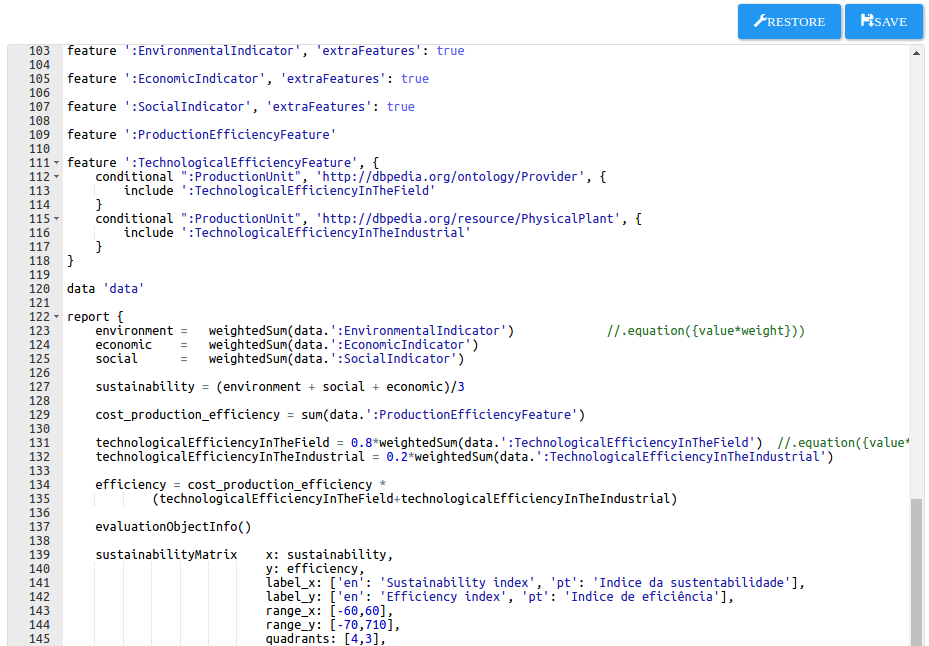
\includegraphics[width=1\columnwidth]{figures/SustenAgro-dsl-editor-2}
\par\end{centering}
\caption{Editor DSL\label{fig:Editor-DSL}}
\end{figure}

O editor da DSL tem compatibilidade com \foreignlanguage{english}{web
components}, tanto os fornecidos pelas bibliotecas integradas no Framework
Decisioner, como com os \foreignlanguage{english}{web components}
do Framework \foreignlanguage{english}{Grails} e adicionalmente podem
ser definidos \foreignlanguage{english}{web components }especializados.
\selectlanguage{english}%

\section{Web components\label{sec:Web-components}}

Web Component\foreignlanguage{brazil}{s }\footnote{\selectlanguage{brazil}%
Site oficial de \foreignlanguage{english}{web components} \url{https://www.webcomponents.org/introduction}\selectlanguage{brazil}%
}\foreignlanguage{brazil}{ é um conjunto de APIs padrão para definir
novas tags }HTML\foreignlanguage{brazil}{ personalizadas, reutilizáveis
e encapsuladas para o uso em páginas ou aplicações web. O framework
Grails também disponibiliza o uso de layout templates para implementar
partes reusáveis de uma view (página HTML). Com essas duas tecnologias,
é possível a criação de componentes (ou widgets) reusáveis da UI. }

\selectlanguage{brazil}%
Para suportar a geração de diferentes tipos de SADs, foi necessário
disponibilizar vários tipos de widgets que permitissem visualizar
e editar diferentes tipos de dados. Para relacionar os \foreignlanguage{english}{web
components} com o conhecimento dos especialistas, modelou-se, na ontologia
Decisioner, os \foreignlanguage{english}{data-types} que permitem
relacionar os tipos de dados com widgets específicas (capazes de edita-los),
usadas nas \foreignlanguage{english}{web UIs} dos SADs gerados. Os
dados das Features dos SADs podem ser de vários tipos e, para cada
tipo, existe uma widget apropriada para visualiza-o. Por exemplo,
para representar uma propriedade de tipo numérico discreto é possível
usar uma widget visual tipo \foreignlanguage{english}{spinner}.

Nos relatórios, os especialistas devem contar com widgets para apresentar
seus resultados em vários formatos, como tabelas, mapas, matriz de
sustentabilidade, etc. Essas widgets podem ser específicas para um
tipo de SAD em particular. Por isso, além do framework contar com
uma biblioteca de widgets prontas, deve ser possível adicionar novas
widgets facilmente. Ao usar padrões, como para Web Components, o framework
permite a fácil inclusão de widgets novas. Não se espera que os especialistas
de domínio criem essas widgets, mas sim que seja fácil para eles consegui-las
de desenvolvedores independentes (que só precisam conhecer o padrão
para Web Components e os requisitos da widget). 

O framework Decisioner tem uma biblioteca de \foreignlanguage{english}{web
components} (widget) construída usando o\foreignlanguage{english}{
web framework Bootstrap }\footnote{\url{http://getbootstrap.com/}},
que conta com diversos componentes básicos para a geração das Web
UI. A maioria deles foi definida usando as \foreignlanguage{english}{layout
templates} do framework \foreignlanguage{english}{Grails}, por ser
mais fácil de programar. Atualmente, apenas dois componentes usam
Web Components.
\selectlanguage{english}%

\section{Web UI}

\selectlanguage{brazil}%
A \foreignlanguage{english}{Web UI} é uma interface web de usuário
responsável por toda a interação com o usuário final. Ela permite
apresentar e editar as informações do SAD, gerar as análises e visualizar
os resultados na web ou em relatórios impressos. O mais importante
é que ela é gerada automaticamente pelo DSL Interpreter, usando a
DSL e ontologias particulares a cada SAD. 

Parte da Web UI é igual para todos os SADs, como formulários de login.
O resto dela é gerado com a ajuda dos \foreignlanguage{english}{Web
Components.} Eles são relacionadas aos tipos de dados existentes no
sistema, por meio da ontologia Decisioner. Por exemplo, dados podem
ser dos tipos numérico contínuo, numérico discreto, percentagem, booleano,
categóricos ou alfanumérico. Dada essa diversidade, os tipos de dados
foram modelados em ontologias com a finalidade de permitir a adaptação
automática (ou semiautomática) da interface às mudanças dos conceitos
do domínio.

Mudanças no layout geral podem ser feitas também através da edição
das \foreignlanguage{english}{Cascading Style Sheets (CSS \nomenclature{CSS}{Cascading Style Sheets})}
do Decisioner. É esperado que, quando da instalação do sistema, técnicos
de informática façam uma customização do sistema para adequá-lo aos
padrões de apresentação da instituição. Eles também devem incluir
qualquer Web Component (widget) necessário mas não disponível por
default no Decisioner. 

A figura \ref{fig:Web-UI} apresenta uma Web UI que foi gerada automaticamente,
a partir da ontologia e das definições na DSL do SAD SustenAgro. Nela
são apresentados vários tipos de \foreignlanguage{english}{Web Components}
que demostram o suporte a diferentes tipos de dados.

\begin{figure}[H]
\begin{centering}
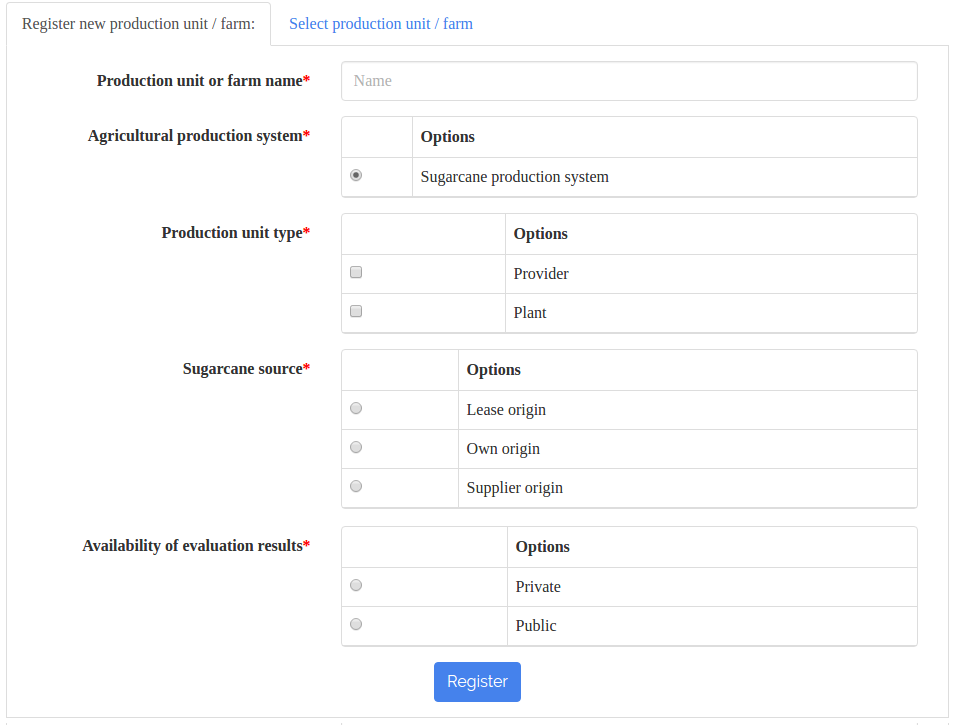
\includegraphics[width=1\columnwidth]{figures/SustenAgro-tool}
\par\end{centering}
\caption{\foreignlanguage{english}{Web UI \foreignlanguage{brazil}{com} web components\label{fig:Web-UI}}}
\end{figure}

\selectlanguage{english}%

\section{DSL Interpreter}

\selectlanguage{brazil}%
O DSL Interpreter é o principal modulo do framework Decisioner. A
sua principal funcionalidade é a interpretação das \foreignlanguage{english}{DSLs}.
Ele executa cada uma das instruções da DSL, vinculando dados e informação,
das ontologias ou fornecidos pelos usuários finais, aos \foreignlanguage{english}{web
components} com a finalidade de gerar as Web \foreignlanguage{english}{UIs}.

Para interagir com os dados da ontologia e apresenta-los na linguagem
dos especialistas, foi necessário criar, no DSL Interpreter, uma camada
de consulta de dados na \foreignlanguage{english}{triplestore} para
simplificar as consultas SPARQL (Figura \ref{fig:Arquitetura-do-Decisioner-Core}).
Esta camada, Sparql Simplifier, foi desenvolvida como uma solução
eficiente para a recuperação de informações semânticas de um domínio
de conhecimento usando um formato simplificado. 

O componente \foreignlanguage{english}{DSL Interpreter} processa
as instruções dos especialistas na linguagem Decisioner DSL. Foram
utilizadas técnicas padrões para a criação de DSLs usando a linguagem
\foreignlanguage{english}{Groovy\citep{dearle2015groovy},} o que
facilitou a definição das \foreignlanguage{english}{DSLs}.

Finalmente, o DSL \foreignlanguage{english}{Interpreter} usa o \foreignlanguage{english}{UI
Renderer} para renderizar dinamicamente as Web \foreignlanguage{english}{UIs}
usando os Web \foreignlanguage{english}{Components.} Esse processo
é repetido toda vez que usuários solicitam uma \foreignlanguage{english}{View}
de um SAD. A figura \ref{fig:Arquitetura-do-Decisioner-Core} apresenta
o DSL Interpreter e os outros módulos com os quais ele se conecta.

\begin{figure}[H]
\begin{centering}
\includegraphics[width=0.7\columnwidth]{\string"figures/Decisioner Core Architecture\string".eps}
\par\end{centering}
\caption{Arquitetura do DSL Interpreter.\label{fig:Arquitetura-do-Decisioner-Core}}
\end{figure}

A figura \ref{fig:Arquitetura-do-Decisioner-Core} também representa
a parte computacional do método proposto nesta pesquisa para definir
SADs. O método consiste em representar o conhecimento dos especialistas
em ontologias da web semântica e complementar com uma DSL que descreve
os conceitos de \foreignlanguage{english}{evaluation object} com \foreignlanguage{english}{features},
método de avaliação e relatório de resultados, permitindo desta maneira
definir o SAD por parte dos especialistas.

\section{Considerações finais}

Neste capítulo foram apresentados os principais componentes do Framework
Decisioner, existem características dele como o gerenciamento de usuários
e segurança que foram desenvolvidos, mas não se especificaram porque
não contribuíram de maneria relevante ao desenvolvimento da pesquisa.

O desenvolvimento do Framework Decisioner foi realizado simultaneamente
com o SAD SustenAgro, devido a que era necessário uma instancia para
validar se as funcionalidades foram implementadas corretamente. O
processo teve dificuldades para separar os dois desenvolvimentos pois
tinha componentes em comum, que a partir de um processo iterativo,
foram organizando-se e permitindo separar os dois sistemas.

Não foi possível instanciar outro sistema no Decisioner durante o
desenvolvimento do mestrado, mas atualmente encontra-se em andamento
a implementação do SAD Nano-Tec como segunda instancia do Framework
Decisioner. O que permitirá generalizar ainda mais e servir como um
caso de uso adicional para validar as hipóteses em outros domínios.
Esta arquitetura foi validada por meio da instanciação do SAD SustenAgro,
o que permite validar se realmente funcionam cada uma das características
aqui descritas.

No capítulo seguinte será apresentado o SAD SustenAgro, gerado como
primeiro caso de uso deste Framework, e depois será apresentado o
processo de avaliação que formaliza a avaliação deste sistema.


